\documentclass[t, notes, xcolor=table]{beamer}

\usepackage{wrapfig}
\usepackage{float}
% For tabs in verbatim
\usepackage{fancyvrb}

% Adjust position of the image
\usepackage[export]{adjustbox}

% set fonts
\usefonttheme{professionalfonts} % using non standard fonts for beamer
\usepackage{txfonts,mathptmx}

% set indend spacing for first and second level indentation
\setlength{\leftmargini}{0.5cm}
\setlength{\leftmarginii}{0.5cm}
\setlength{\leftmarginiii}{0.5cm}

% Set circles for bullets 
\setbeamertemplate{itemize items}[circle]

% colors
\usepackage{xcolor}

% multiple columns
\usepackage{multicol}

% todo lists
\usepackage{pifont}
\usepackage{amssymb}

% increase space between text and frame name
\addtobeamertemplate{frametitle}{}{\vspace{0.5em}}

%Information to be included in the title page:
\title{Using Functions and Tasks}
\author{Nikola Petrovic}
\institute{University of Belgrade, School of Electrical Engineering}
\date{2022}



\begin{document}

\frame{\titlepage}

%%%%%%%%%%%%%%%%%%%%%%%%%%%%%%%%%%%%%%%%%%%%%%%%%%%%%%%%%%%%
\begin{frame}
\frametitle{Module Objective}
In this module we will write Verilog subroutines to encapsulate functionality making your code more readable and reusable.
\newline

\textbf{Topics:}
\begin{itemize}
\item Verilog Subroutine Introduction
\item Functions - Declaration and Calling
\item Tasks - Declaration and Calling
\item Issues with Functions and Tasks
\end{itemize}

\end{frame}
\note{
\scriptsize{
Out objective is to effectively use subroutines to encapsulate functionality and thus to make our code more readable and reusable. To do that, we need to know what subroutines are available and how to use them.


}
}

%%%%%%%%%%%%%%%%%%%%%%%%%%%%%%%%%%%%%%%%%%%%%%%%%%%%%%%%%%%%
\begin{frame}
\frametitle{Verilog Subroutines Introduction}
Subroutines:
\begin{itemize}
\item Encapsulate code that might otherwise be duplicated.
\item Contain statements that execute in sequence.
\end{itemize}

\begin{multicols}{2}
Function subroutines:
\scriptsize{
\begin{itemize}
\item Have one or more inputs and return a single value.
\item Are invoked as an expression term.
\end{itemize}
}
\vfill
\columnbreak
\normalsize{
Task subroutines:
}
\scriptsize{
\begin{itemize}
\item Have zero or more input/outputs.
\item Are invoked as a procedural statement.
\end{itemize}
}
\end{multicols}
\begin{figure}
    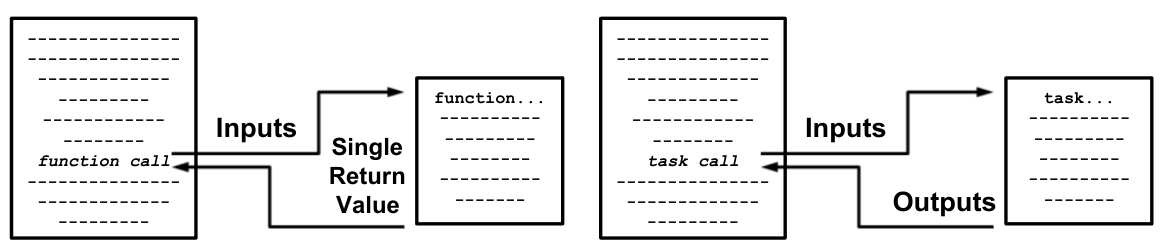
\includegraphics[width=0.95\textwidth]{img/10_subroutines.png}
\end{figure}
\end{frame}
\note{
\scriptsize{
Let's first examine the purpose of subroutines:
\begin{itemize}
\item We can think of a subroutine as a level of hierarchy, or structure, in sequential code. We can use subroutines to encapsulate some frequently used code in one place where we can more easily manage it. We can provide this ode with inputs, wo which we assign values as we invoke the subroutines. These input values can flexibly direct the subroutine to perform slightly for each invocation.

Encapsulating sequential code in subroutines is similar to encapsulating design units in modules.
\end{itemize}

}
}

%%%%%%%%%%%%%%%%%%%%%%%%%%%%%%%%%%%%%%%%%%%%%%%%%%%%%%%%%%%%
\begin{frame}[fragile]
\frametitle{Declaring Functions}
\scriptsize{
Function are declared only within a module. They start with \textcolor{purple}{function} keyword and ends with \textcolor{purple}{endfunction} keyword.
\newline

\textbf{Syntax:}
}
\tiny{
\begin{Verbatim}[commandchars=\\\{\}, tabsize=2]
\textcolor{purple}{function} [automatic] [signed] [range_or_type] function_identifier;
	tf_input_declaration;
	\{tf_input_declaration;\}
	\{block_item_declaration\}
	function_statement
\textcolor{purple}{endfunction}
\end{Verbatim}
}
\scriptsize{
\textbf{Alternative Syntax:}
}
\tiny{
\begin{Verbatim}[commandchars=\\\{\}, tabsize=2]
\textcolor{purple}{function} [automatic] [signed] [range_or_type] function_identifier;
	(function_port_list);
	\{block_item_declaration\}
	function_statement
\textcolor{purple}{endfunction}
\end{Verbatim}
}
\scriptsize{

\vfill
Function syntax without and with the function port list:
}
\begin{figure}
    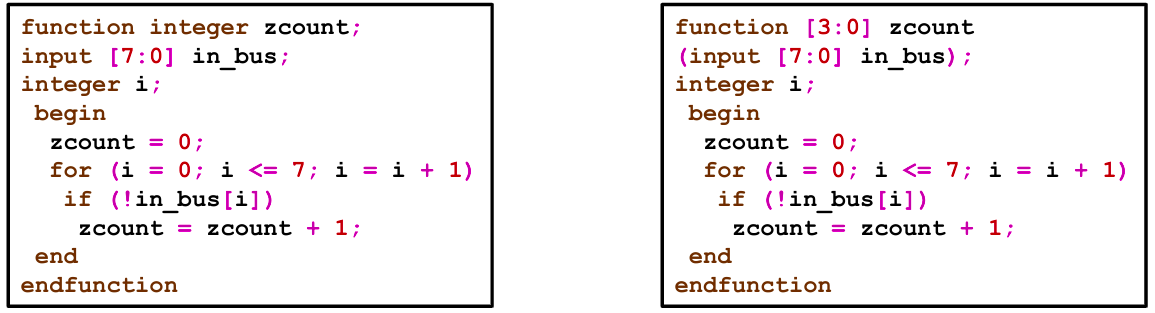
\includegraphics[width=0.95\textwidth]{img/10_function.png}
\end{figure}

\end{frame}
\note{
\tiny{
We declare a function only within a module. The declaration starts with the \textit{function} keyword.
\newline

Functions are by default \textbf{static}. That means that exactly one copy of the function variables exists. All calls to the function utilize that one set of function variables, thus calls to static functions are generally not recursive. External code can access static function variables using hierarchical references. Verilog 2001 added the \textit{automatic} declaration. Automatic functions create a new temporary set of their variables for each call. Automatic functions can be recursive. External code cannot access automatic function variables. The \textit{return} type defaults to a single bit. We can alternatively specify \textit{integer, real, realtime, time} or a vector range. A vector is by default not signed. We can declare the vector \textit{signed}. The signed declaration is a Verilog 2001 feature.
\newline

A function must have at least one input port and most have no output and no inout ports. We can declare input ports using either syntax. With the \textit{function port list} syntax, we can prefix port attributes. The input port defaults to the single bit. We can alternatively specify \textit{integer, real, realtime, time} or vector range. A venctor is by default not signed. We can declare the vector \textit{signed}. The signed declaration is a Verilog 2001 feature.
\newline

We can declare additional block items. We cannot declare module items. For example, we can declare variables but not nets!
\newline

A function declaration contains a statement. The statement may be a statement block, for example grouped between \textbf{begin} and \textbf{end} keywords. Functions cannot invoke the scheduler. That means that function assignments are always blocking and functions always execute completely and instantly.
\newline

Function can have side-effects, for example, a function can assign to a module variable but not to a module net. For a function to have side-effect is undesirable programming practice. Instead, declare the function return vector sufficiently wide to hold all data we need to return , then deconstruct the vector value as needed upon return.
\newline

A function declaration ends with the \textit{endfunction} keyword.

}
}

%%%%%%%%%%%%%%%%%%%%%%%%%%%%%%%%%%%%%%%%%%%%%%%%%%%%%%%%%%%%
\begin{frame}[fragile]
\frametitle{Calling Functions}
We call a function as an expression term:
\begin{Verbatim}[commandchars=\\\{\}, tabsize=2]
\textcolor{purple}{		function_identifier (expression \{, expression\})}
\end{Verbatim}
\begin{figure}
    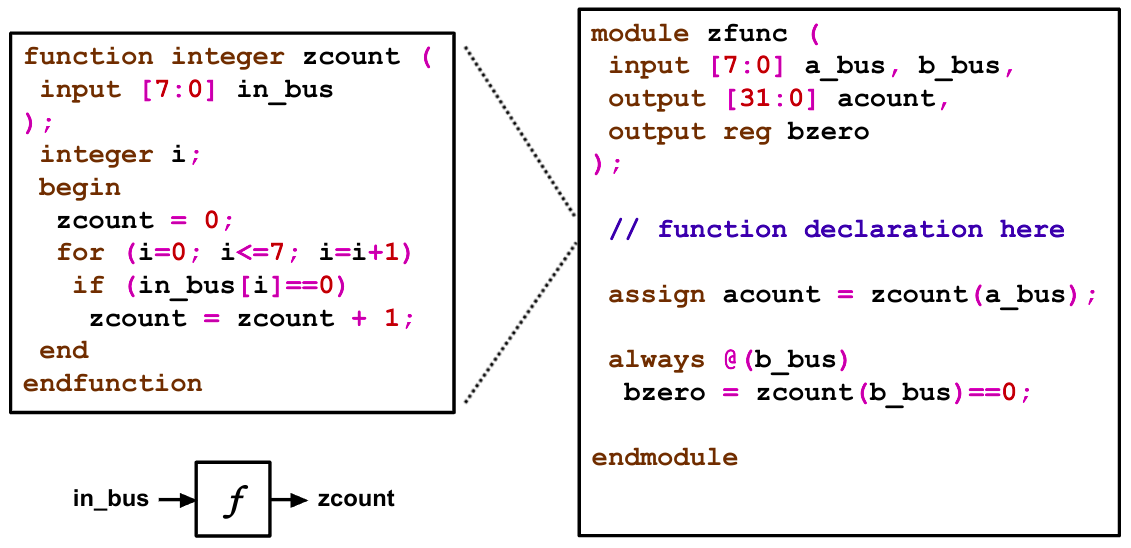
\includegraphics[width=0.95\textwidth]{img/10_function_call.png}
\end{figure}
\end{frame}
\note{
\scriptsize{
We call a function as an expression term. The simulator assigns the values of the argument expressions to the input ports in the order in which they appear in the call.
\newline

When the function completes, the simulator uses the value of the function name variable where the function call appears in the calling expression. Functions return a single value that we use as an operand in an \textit{rvalue} expression. An rvalue expression is one that may appear only on the right side of an assignment - we cannot assign a value to an rvalue expression. If the function never completes, for example, it executes a loop that loops forever, it never returns and simulator "hangs".
\newline

In this example, the \textit{zcount} function returns an integer value representing the number of bits of the \textit{in\_bus} port that are zero. It returns a value between 0 and 8. The continuous assignment call assigns the returned value to the \textit{acount} module output port. The procedural assignment call uses the function return value as an operand in a comparison expression.

}
}

%%%%%%%%%%%%%%%%%%%%%%%%%%%%%%%%%%%%%%%%%%%%%%%%%%%%%%%%%%%%
\begin{frame}
\frametitle{Constant Functions}
\scriptsize{
\begin{multicols}{2}
Verilog-1995 allows simple constant expressions for defining limits for vectors, replicates, etc.

\begin{itemize}

\item Verilog-2001 allows limits to be defined by constant functions.
\item Function value must be calculable at elaboration. Usually inputs are constants.
\item Greater flexibility for scalable reusable models.
\item Multiple limits can be derived from a single constant.
\end{itemize}
\vfill
\columnbreak
\begin{figure}
    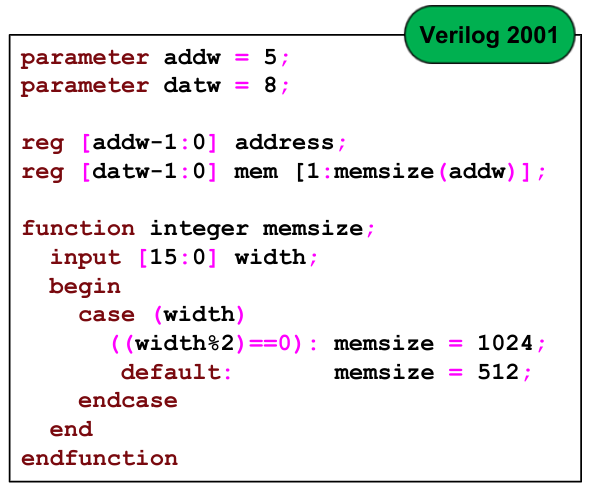
\includegraphics[width=0.45\textwidth]{img/10_function_const.png}
\end{figure}
\end{multicols}
}
\end{frame}
\note{
\tiny{
Verilog 1995 module parameter values must be constant expressions, which are limited to operations on literals and previously declared module parameters.
\newline

Verilog 2001 permits us to use a constant function call anywhere we are required to use a constant expression.
\newline

The standard lists restrictions upon a constant function calls:
\begin{itemize}
\item Cannot be placed within any generate scope
\item Cannot contain hierarchical references
\item Cannot contain system function calls 
\item Ignores system task calls (but will execute \$display in sumulator but not in elaborator)
\item Cannot themselves make constant function calls in any context requiring constant expressions. Can otherwise make constant function calls to functions local to containing module.
\item Can access only functions and module parameters and nothing else declared outside the function definition
\item Module parameters must be previously assigned. Use of \textit{defparam} can produce undefined results.
\end{itemize}

}
}

%%%%%%%%%%%%%%%%%%%%%%%%%%%%%%%%%%%%%%%%%%%%%%%%%%%%%%%%%%%%
\begin{frame}
\frametitle{Declaring Tasks}
\begin{itemize}
\item \textcolor{purple}{Task} is declared only within a module
\item Declaration starts with \textcolor{purple}{task} and ends with \textcolor{purple}{endtask} keyword
\end{itemize}
\begin{figure}
    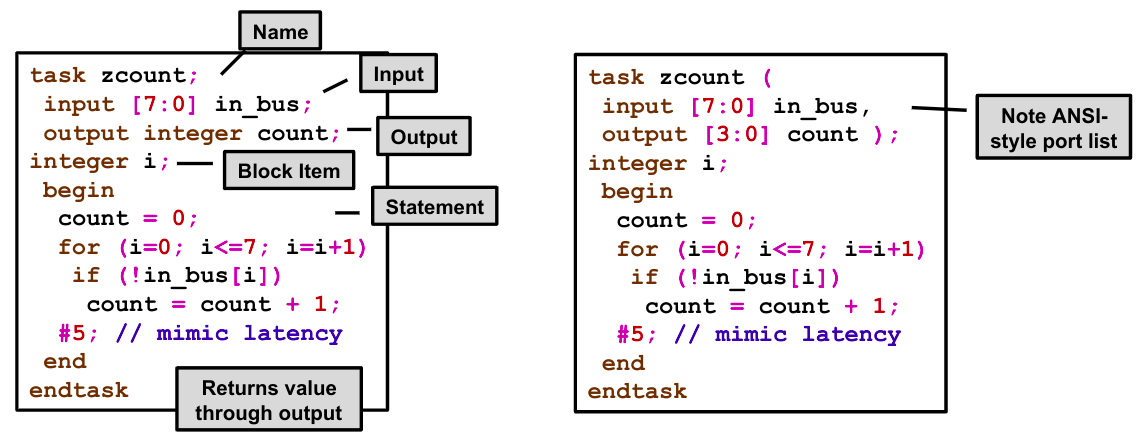
\includegraphics[width=0.95\textwidth]{img/10_task.png}
\end{figure}
\end{frame}
\note{
\tiny{
We declare a \textit{task} only within a module. Declaration starts with \textcolor{purple}{task} and ends with \textcolor{purple}{endtask} keyword.
\newline

Tasks are by default \textit{static}. That means that exactly one copy of the task variables exists. All calls to the task utilize that one set of task variables, thus calls to static tasks are generally not re-enter able. External code can access static task variables using hierarchical references. Verilog 2001 added te \textit{automatic} declaration. Automatic tasks create a new temporary set of their variables for each call. Automatic tasks are re-enter able. External code cannot access automatic task variables.
\newline

A task can have any number of \textit{input, output} or \textit{inout} ports. We can declare the ports using either syntax. Either syntax accepts port attributes. The port type defaults to a single bit. We can alternatively specify \textit{integer, real, realtime, time} or a vector range. A vector is by default unsigned. We can declare vector \textit{signed}. The \textit{signed} declaration is a Verilog 2001 feature.
\newline

We can declare additional block items. We cannot declare module items. For example, we can declare variables but not nets.
\newline
A task declaration contains a statement. The statement may be a statement block, for example grouped between the \textit{begin} and \textit{end} keywords. Tasks can invoke the scheduler. That means task assignments can be blocking or non-blocking and tasks can delay their completion for any amount of time. We can rewrite as a function any task that does not invoke the scheduler.
\newline

Tasks can have side effects, for example, a task can assign to a module variable but not to a module net. For a task to have side effect is a very useful feature and common programming practice.

}
}

%%%%%%%%%%%%%%%%%%%%%%%%%%%%%%%%%%%%%%%%%%%%%%%%%%%%%%%%%%%%
\begin{frame}[fragile]
\frametitle{Calling (Enabling) Tasks}

We call (enable) a task as a statement:
\scriptsize{
\begin{Verbatim}[commandchars=\\\{\}, tabsize=2]
\textcolor{purple}{		hierarchical_task_identifier [(expression \{, expression\})];}
\end{Verbatim}
}
\begin{figure}
    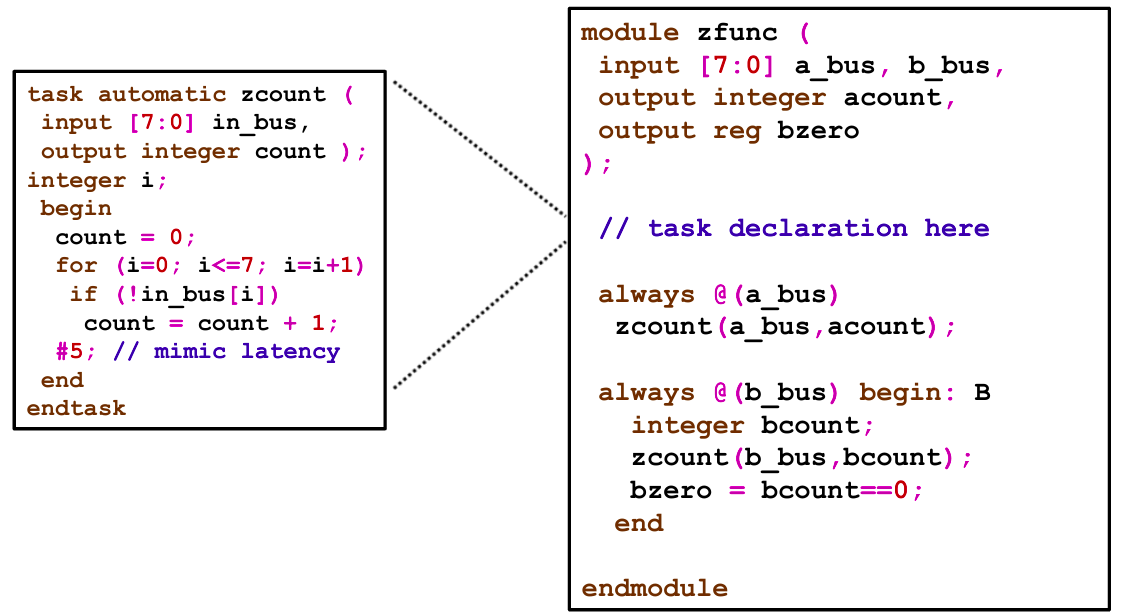
\includegraphics[width=0.95\textwidth]{img/10_task_call.png}
\end{figure}
\end{frame}
\note{
\scriptsize{
We call a task as a procedural statement. The simulator assigns the values of the input and inout argument expressions to their ports. The standard refers to these "calls" as \textit{enables} to remind us that a task can consume simulation time and thus can execute concurrently with other procedures.
\newline

When the task completes,
the simulator assigns the values of the output and inout ports to their \textit{lvalue} expression arguments. An lvalue expression may appear on the left side of an assignment - we can assign a value to an lvalue expression. If the task never completes, for example, in a loop that loops forever, it never returns and its calling procedure cannot continue. However, if the task "consumes" time, procedures other than the calling procedure can execute.
\newline

In this example, the \textit{zcount} task returns an integer value representing the number of bits of the \textit{in\_bus} port that are zero. it returns a value between 0 and 8. Both task enables are procedural statements. As both procedures can concurrently have the task enabled, the task variables must be automatic variables so that each procedure gets their own copy.

}
}

%%%%%%%%%%%%%%%%%%%%%%%%%%%%%%%%%%%%%%%%%%%%%%%%%%%%%%%%%%%%
\begin{frame}
\frametitle{Tasks without Timing controls}
\begin{itemize}
\item Tasks can use the scheduler with delays and timing controls.
\item We can rewrite a task that doesn't use a scheduler as a function:
\end{itemize}
\begin{figure}
    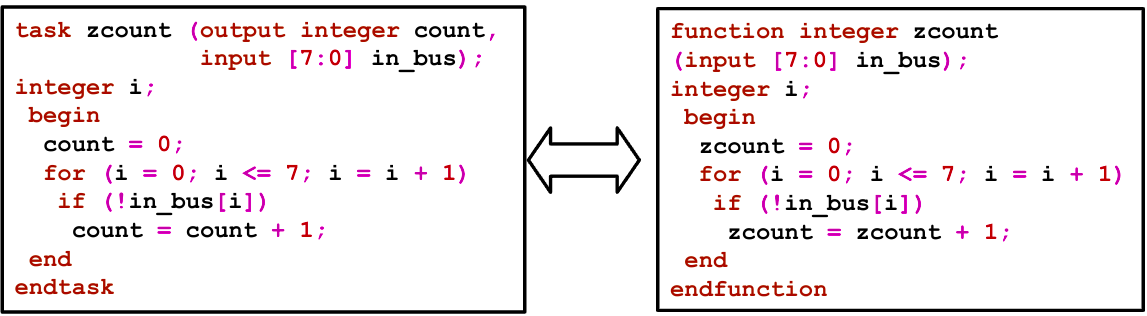
\includegraphics[width=0.95\textwidth]{img/10_task_func.png}
\end{figure}
\end{frame}
\note{
Tasks can invoke the scheduler. That means task assignments can be blocking or non-blocking and tasks can delay their completion for any amount of time. A task that does not invoke a scheduler can be rewritten as a function.

}

%%%%%%%%%%%%%%%%%%%%%%%%%%%%%%%%%%%%%%%%%%%%%%%%%%%%%%%%%%%%
\begin{frame}
\frametitle{Disabling Tasks}
\scriptsize{
\begin{multicols}{2}
We can disable a task (force it to exit):
\begin{itemize}
\item In this example, detection of an interrupt disables any currently running \textit{cpu\_driver} task.
\item Future statements can again enable the \textit{cpu\_driver} task.
\end{itemize}
\vfill
\textcolor{red}* We can also disable named blocks.
\columnbreak
\begin{figure}
    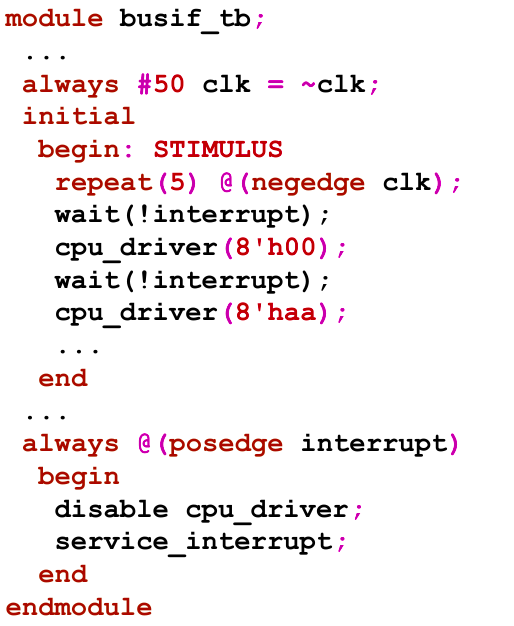
\includegraphics[width=0.45\textwidth]{img/10_task_disable.png}
\end{figure}
\end{multicols}
}
\end{frame}
\note{
\scriptsize{
The \textbf{disable} statement terminates activity associated with the task or named block. We can use it to work around the lack of C-like \textit{break} and \textit{continue} statements. We can use it to behaviourally model asynchronous activity such as interrupts.
\newline

The simulator discontinues any activity associated with the task or named block. If executing the task or named block, it resumes execution with the statement after the task call of after the named block Implementations can choose whether to remove scheduled non-blocking assignments and whether to discontinue procedural continuous assignments, so this can be a source of differences between simulators.


}
}

%%%%%%%%%%%%%%%%%%%%%%%%%%%%%%%%%%%%%%%%%%%%%%%%%%%%%%%%%%%%
\begin{frame}
\frametitle{Issues with Functions and Tasks}

Function and task definitions and declarations are by default static.

\scriptsize{
\begin{itemize}
\item Multiple execution threads within a function or task by default all use the same set of ports and variables.
\item As tasks consume time, we can easily have multiple task calls simultaneously executing.
\item Functions and tasks can recursively call themselves.
\end{itemize}
}

\normalsize{
Function and task arguments are passed by value.
}
\scriptsize{
\begin{itemize}
\item Input argument transition are not visible to the task.
\end{itemize}
}

\normalsize{
A function or task can have side effects.
}
\scriptsize{
\begin{itemize}
\item Can directly access variables in the scope of the module that defines it.
\item Can access (using out-of-module references) any static variable.
\end{itemize}
}

\end{frame}
\note{
\scriptsize{
The following slides explore three characteristics of functions and tasks.
\begin{itemize}
\item The first issues is that by default there is only one copy of a subroutine's variables, so that multiple outstanding calls to the same subroutine clobber each other.
\item The second issue is that arguments are passed and returned by value. The subroutines maintain local variables that get the input values upon invocation. A task cannot observe future transitions on the net or variable arguments from which the passed value derived.
\item The third issue is that subroutines can have side-effects, they can directly access the defining module's nets and variables, and can through out-of-module references access any nets and variables in the simulation. This is not an issues as much as it is a benefit, as it can greatly ease our testbench development effort.
\end{itemize}

}
}

%%%%%%%%%%%%%%%%%%%%%%%%%%%%%%%%%%%%%%%%%%%%%%%%%%%%%%%%%%%%
\begin{frame}
\frametitle{Automatic Tasks: Re-Entering Subroutines}
\scriptsize{
\begin{multicols}{2}
\textbf{Verilog 1995}
\begin{itemize}
\item All tasks and functions are static.
\begin{itemize}
\tiny{
	\item Concurrent task call and recursive function calls must be avoided.
	\item Can cause conflict with internal variables and arguments.
}
\end{itemize}
\end{itemize}

\textbf{Verilog 2001}

\begin{itemize}
\item Can declare tasks and functions to be dynamic using keyword \textit{automatic}.
\item Allows concurrent task calls and recursive function calls.
\begin{itemize}
\tiny{
	\item These declarations cannot be accessed by hierarchical references.
	\item These arguments cannot be updated with non-blocking assignments.
}
\end{itemize}
\end{itemize}
\vfill
\columnbreak
\begin{figure}
    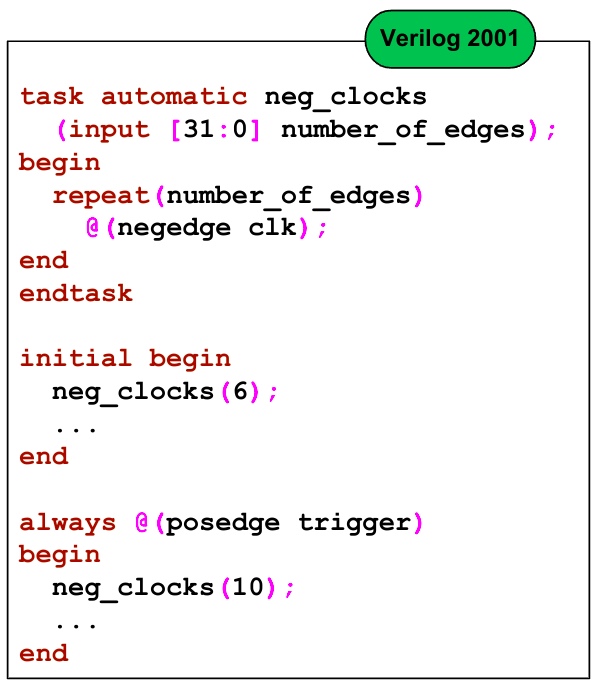
\includegraphics[width=0.45\textwidth]{img/10_task_re_enter.png}
\end{figure}
\end{multicols}
}
\end{frame}
\note{
\scriptsize{
For Verilog 1995 , all subroutines are static. Only one copy of a subroutine arguments and variables exist. Multiple concurrent task calls and recursive function calls all use the same copy of inputs, local variables, and outputs.
\newline

For Verilog 2001, we can declare an automatic subroutine. A separate copy of the subroutine arguments and variables exists for each invocation Multiple concurrent task calls and recursive function calls all use their own copy of inputs, local variables, and outputs. As the automatic arguments and variables exist only for a duration of the subroutine execution, we cannot reference them hierarchically from outside the subroutine, cannot assign them with non-blocking assignments, and cannot use \textit{\$monitor} or \textit{\$strobe} with them.

}
}

%%%%%%%%%%%%%%%%%%%%%%%%%%%%%%%%%%%%%%%%%%%%%%%%%%%%%%%%%%%%
\begin{frame}
\frametitle{Arguments Are Passed by Value}
\scriptsize{
\begin{multicols}{2}
Arguments are passed by value.

\begin{itemize}
\item The simulator assigns expression values to input arguments upon invocation.
\item The simulator assigns output values to output argument variables upon return.
\end{itemize}
\vfill
\columnbreak
\begin{figure}
    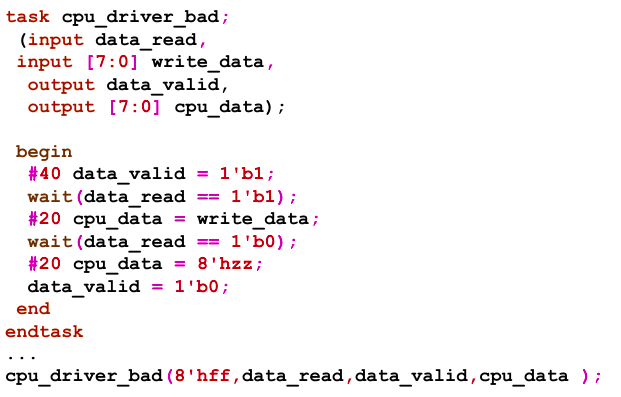
\includegraphics[width=0.45\textwidth]{img/10_value_pass1.png}
\end{figure}
\end{multicols}
}
\begin{figure}
    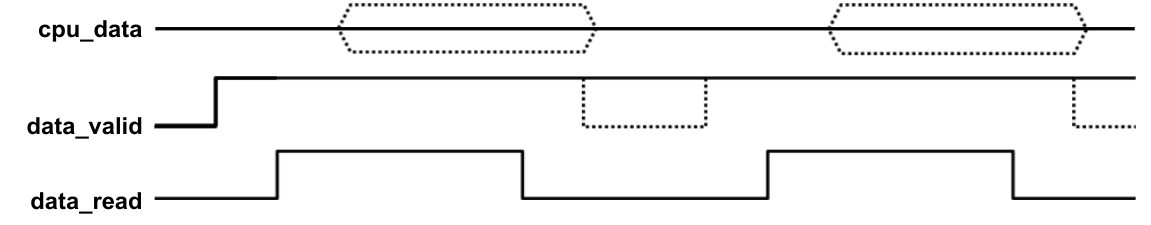
\includegraphics[width=0.95\textwidth]{img/10_value_pass2.png}
\end{figure}
\end{frame}
\note{
\scriptsize{
Subroutine arguments are passed by value.
\begin{itemize}
\item The simulator assigns actual argument values to formal input arguments upon invocation.
\item The simulator assigns output values to output argument variables upon return.
\end{itemize}

The problem with the \textit{cpu\_driver\_bad} task is that the input argument \textit{data\_read} is sampled when the task is called and used throughout the task execution. External changes in \textit{data\_read} are not seen within the task during the lifetime of the task execution. Therefore the task hangs at the firs wait statement.
\newline

Also the assignment to the output argument \textit{data\_valid} is not made - this will only be updated at the end of the task execution, but because the task never completes, \textit{data\_read} is never updated.

}
}

%%%%%%%%%%%%%%%%%%%%%%%%%%%%%%%%%%%%%%%%%%%%%%%%%%%%%%%%%%%%
\begin{frame}
\frametitle{Example: Task with Side-Effects}
\scriptsize{
\begin{multicols}{2}
Subroutines can have "side effects", can directly access items of their declaring module, and can access other design items \textcolor{purple}{hierarchically}.
\begin{itemize}
\item Advantage - Allows encapsulation of a frequently used algorithm or testbench-DUT transaction.
\item Disadvantage - More difficult to reuse the subroutine for other purposes.
\end{itemize}
\vfill
\columnbreak
\begin{figure}
    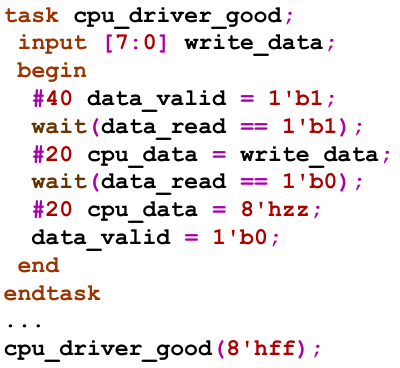
\includegraphics[width=0.45\textwidth]{img/10_task_ex1.png}
\end{figure}
\end{multicols}
}
\begin{figure}
    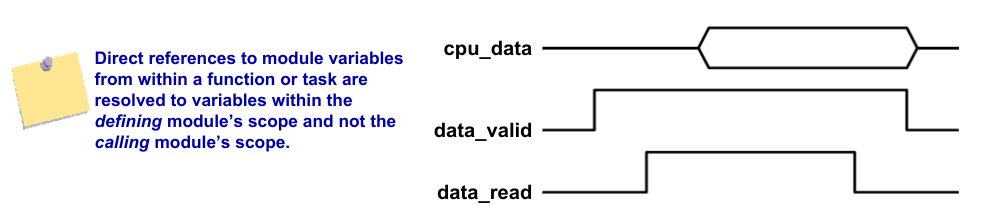
\includegraphics[width=0.95\textwidth]{img/10_task_ex2.png}
\end{figure}
\end{frame}
\note{
\scriptsize{
Subroutines can bypass their ports to read and write directly the variables of the defining module, and other design items by hierarchical reference.
\newline

This feature greatly simplifies our testbench.
\newline

This modified task directly references the \textit{data\_valid} and \textit{data\_read} module variables instead of having their values passed as argument. The \textit{wait} statements inside the task can now detect transitions of the \textit{data\_read} variable and the task will operate correctly.
\newline

Keep in mind that direct subroutine references to module variables are to those within the \textit{defining} module's scope and not the \textit{calling} module's scope.

}
}

%%%%%%%%%%%%%%%%%%%%%%%%%%%%%%%%%%%%%%%%%%%%%%%%%%%%%%%%%%%%
\begin{frame}
\frametitle{Subroutines Can Access Module Variables}
\begin{figure}
    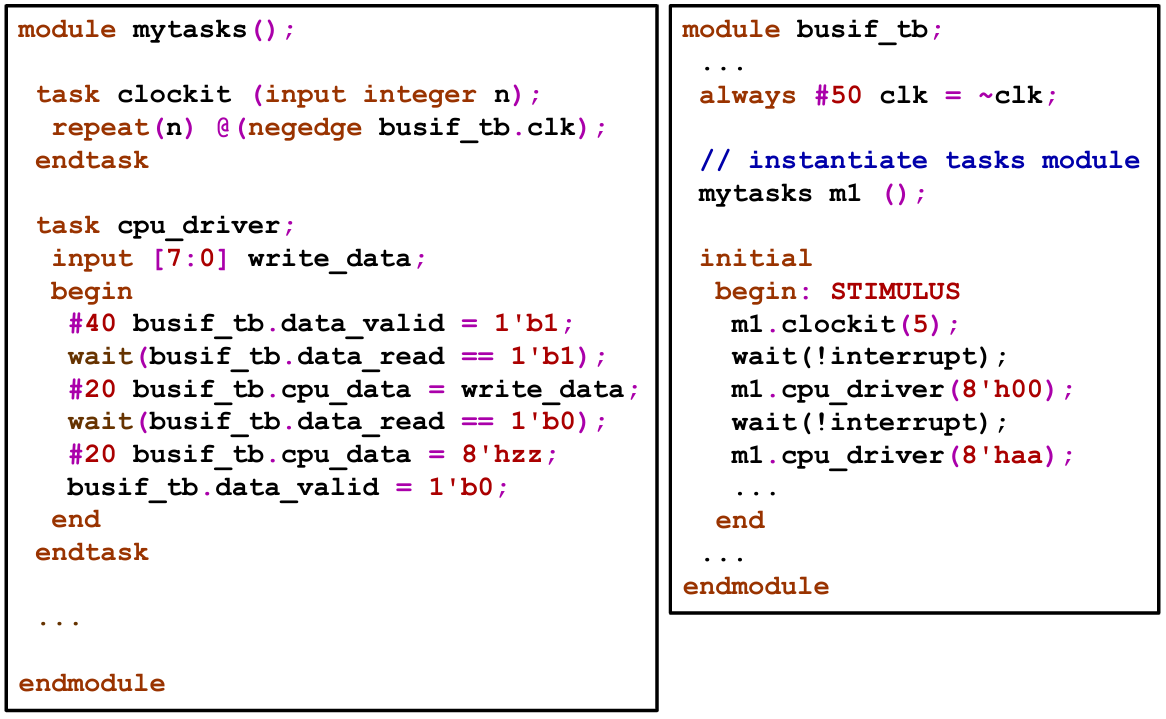
\includegraphics[width=0.95\textwidth]{img/10_sub_access.png}
\end{figure}
\end{frame}
\note{
\scriptsize{
At some point, we can find it convenient to declare a subroutine in one module and call it from another module.
\newline

Every Verilog object has a unique path name that starts at a top-level instance, and using the dot (.) character hierarchy separator, traverses down through instance names to the name of the object. We can use these hierarchical names for any Verilog 1995 object. We are not permitted to use the hierarchical name of a Verilog 2001 automatic subroutine variable.
\begin{itemize}
\item Hierarchical references can be absolute, starting at a top-level instance and traversing a downward path.
\item Hierarchical references can be relative, starting at the scope of the reference and traversing a downward path.
\item Hierarchical references can also be upward, but such references can have only a single instance or a module name, which resolves to the nearest upward instance or module with that name.
\end{itemize}

}
}

%%%%%%%%%%%%%%%%%%%%%%%%%%%%%%%%%%%%%%%%%%%%%%%%%%%%%%%%%%%%
\begin{frame}
\frametitle{Module Summary}
We can now make our code more readable and reusable by encapsulating functionality in Verilog subroutines.
\newline
This module describes:
\begin{itemize}
\item Subroutine Concepts:
\begin{itemize}
	\item Encapsulate code that might otherwise be duplicated.
\end{itemize}
\item Functions:
\begin{itemize}
	\item Have one or more inputs and return a single value through their name.
	\item Are invoked as an expression term.
\end{itemize}
\item Tasks:
\begin{itemize}
	\item Have zero or more input and zero or more outputs.
	\item Are invoked as a procedural statements.
\end{itemize}
\item Issues:
\begin{itemize}
	\item Subroutine variables are by default static.
	\item Subroutine arguments are passed by value.
	\item Subroutine can directly access module nets and variables.
\end{itemize}
\end{itemize}
\end{frame}
\note{
\scriptsize{
After completing this module, we can effectively use subroutines to encapsulate functionality and make our code more readable and reusable. This module described Verilog subroutines known as functions and tasks. It explained where and how to define, them, how to invoke them, and some issues involved with using them.

}
}

%%%%%%%%%%%%%%%%%%%%%%%%%%%%%%%%%%%%%%%%%%%%%%%%%%%%%%%%%%%%
\begin{frame}
\frametitle{Module Review}
\begin{enumerate}
\item Which subroutine(s) can contain timing controls?
\item A call to which subroutine(s) can appear outside procedures?
\item What is the default type of a subroutine port?
\item By which method are subroutine arguments passed (value, pointer, reference)?
\end{enumerate}
\end{frame}
\note{
\scriptsize{
\begin{enumerate}
\item Which subroutine(s) can contain timing controls?
\begin{itemize}
\scriptsize{
	\item Only a task can contain timing controls. A function cannot invoke the scheduler in any way.
}
\end{itemize}
\item A call to which subroutine(s) can appear outside procedures?
\begin{itemize}
\scriptsize{
	\item We use a function call as a term of an expression, so a function call can appear on the right side of a continuous assignment.
}
\end{itemize}
\item What is the default type of a subroutine port?
\begin{itemize}
\scriptsize{
	\item A subroutine port is by default a single-bit reg. We can declare it as any variable type. Subroutines cannot declare nets.
}
\end{itemize}
\item By which method are subroutine arguments passed (value, pointer, reference)?
\begin{itemize}
\scriptsize{
	\item Subroutine arguments are passed by value.
}
\end{itemize}
\end{enumerate}

}
}

%%%%%%%%%%%%%%%%%%%%%%%%%%%%%%%%%%%%%%%%%%%%%%%%%%%%%%%%%%%%
\begin{frame}
\frametitle{Module Exercise}
Write a task to accept a 32-bit input argument address and place that address on the "abus" and increment the address through a total of four cycles. The task also controls the "sel" signal. Refer to the diagram.
\begin{figure}
    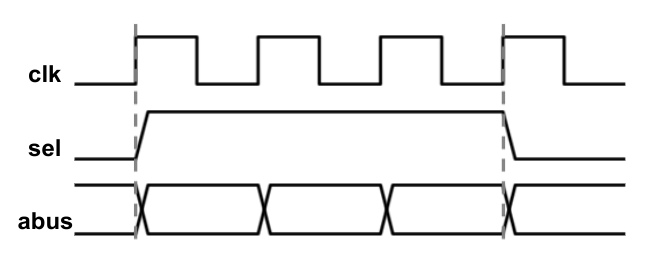
\includegraphics[width=0.55\textwidth]{img/10_ex.png}
\end{figure}
\end{frame}
\note{
\begin{figure}
    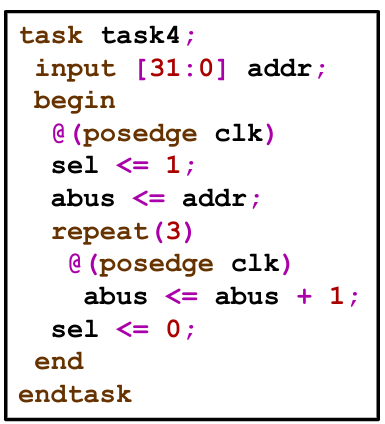
\includegraphics[width=0.45\textwidth]{img/10_ex_sol.png}
\end{figure}
}

%%%%%%%%%%%%%%%%%%%%%%%%%%%%%%%%%%%%%%%%%%%%%%%%%%%%%%%%%%%%
\begin{frame}
\frametitle{Lab}
Lab 11-1: Modeling the Counter Using Functions
\begin{itemize}
\item Encapsulate counter design combinational behaviours in a function.
\end{itemize}

Lab 11-2: Modeling the Memory Test Block Using Tasks
\begin{itemize}
\item Encapsulate memory test procedural behaviours in tasks.
\end{itemize}
\begin{figure}
    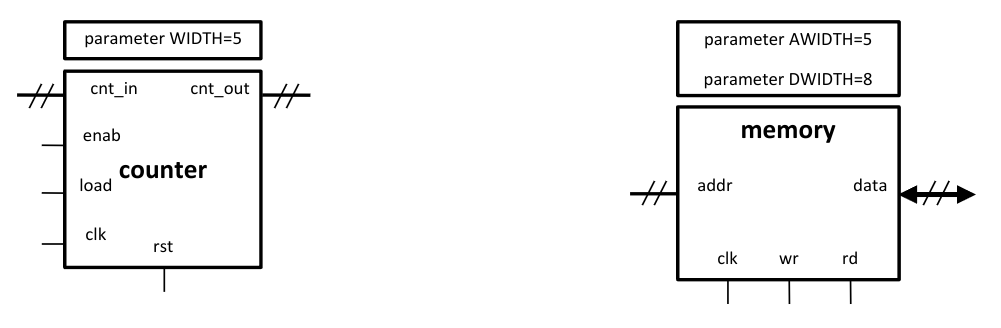
\includegraphics[width=0.75\textwidth]{img/10_lab.png}
\end{figure}
\end{frame}

%%%%%%%%%%%%%%%%%%%%%%%%%%%%%%%%%%%%%%%%%%%%%%%%%%%%%%%%%%%%
\begin{frame}
\frametitle{Test You Understanding - 1}
Which one or more types can you use for a task or function port?
\begin{itemize}
\item[$\square$] 
\item[$\square$] 
\item[$\square$] 
\item[$\square$] 
\end{itemize}
\end{frame}
\note{

}

%%%%%%%%%%%%%%%%%%%%%%%%%%%%%%%%%%%%%%%%%%%%%%%%%%%%%%%%%%%%
\begin{frame}
\frametitle{Test You Understanding - 1}
Which one or more types can you use for a task or function port?
\begin{itemize}
\item[$\square$] reg
\item[$\square$] integer
\item[$\square$] real
\item[$\square$] time
\end{itemize}
\end{frame}
\note{
Which one or more types can you use for a task or function port?
\begin{itemize}
\item[$\boxtimes$] reg
\item[$\boxtimes$] integer
\item[$\boxtimes$] real
\item[$\boxtimes$] time
\end{itemize}
}

%%%%%%%%%%%%%%%%%%%%%%%%%%%%%%%%%%%%%%%%%%%%%%%%%%%%%%%%%%%%
\begin{frame}
\frametitle{Test You Understanding - 2}
Your task or function definition declare nets. True or false?
\begin{itemize}
\item[$\square$] True
\item[$\square$] False
\end{itemize}
\end{frame}
\note{
Your task or function definition declare nets. True or false?
\begin{itemize}
\item[$\square$] True
\item[$\boxtimes$] False
\end{itemize}
}

%%%%%%%%%%%%%%%%%%%%%%%%%%%%%%%%%%%%%%%%%%%%%%%%%%%%%%%%%%%%
\begin{frame}
\frametitle{Test You Understanding - 3}
Which one or more things you NOT do within a functions?
\begin{itemize}
\item[$\square$] Enable a task
\item[$\square$] Declare an output argument
\item[$\square$] Make non-blocking assignments
\item[$\square$] Utilize timing controls
\end{itemize}
\end{frame}
\note{
Which one or more things you NOT do within a functions?
\begin{itemize}
\item[$\boxtimes$] Enable a task
\item[$\boxtimes$] Declare an output argument
\item[$\boxtimes$] Make non-blocking assignments
\item[$\boxtimes$] Utilize timing controls
\end{itemize}
}

%%%%%%%%%%%%%%%%%%%%%%%%%%%%%%%%%%%%%%%%%%%%%%%%%%%%%%%%%%%%
\begin{frame}
\frametitle{Test You Understanding - 4}
You pass task or function arguments by passing:
\begin{itemize}
\item[$\square$] a reference to a net, variable, or constant
\item[$\square$] a pointer to a net, variable, or constant
\item[$\square$] the value of a net, variable, or constant
\end{itemize}
\end{frame}
\note{
You pass task or function arguments by passing:
\begin{itemize}
\item[$\square$] a reference to a net, variable, or constant
\item[$\square$] a pointer to a net, variable, or constant
\item[$\boxtimes$] the value of a net, variable, or constant
\end{itemize}
}

%%%%%%%%%%%%%%%%%%%%%%%%%%%%%%%%%%%%%%%%%%%%%%%%%%%%%%%%%%%%
\begin{frame}
\frametitle{Test You Understanding - 5}
Which one or more things can you NOT do with automatic task variables?
\begin{itemize}
\item[$\square$] Reference them in intra-assignment event controls
\item[$\square$] Make blocking assignments to them
\item[$\square$] Dump them to a waveform database
\item[$\square$] Make non-blocking assignments to them
\end{itemize}
\end{frame}
\note{
Which one or more things can you NOT do with automatic task variables?
\begin{itemize}
\item[$\boxtimes$] Reference them in intra-assignment event controls
\item[$\square$] Make blocking assignments to them
\item[$\boxtimes$] Dump them to a waveform database
\item[$\boxtimes$] Make non-blocking assignments to them
\end{itemize}
}





\end{document}
